\documentclass{sig-alt-release2}
\usepackage{times}
\usepackage[usenames]{color}
\sloppypar

% Title Page
\title{Streaming of 3D Progressive Meshes}
\numberofauthors{1}
\author{\alignauthor Wei Cheng\\
\affaddr{School of Computing,National University of Singapore}\\
\email{chengwe2@comp.nus.edu.sg}}
\begin{document}
\conferenceinfo{MM'08,}{October 26--31, 2008, Vancouver, British Columbia, Canada.}
\CopyrightYear{2008}
\crdata{978-1-60558-303-7/08/10}
\maketitle
\begin{abstract}
%The 3D meshes are increasingly available over the network.
%To reduce the waiting time when downloading
%high resolution 3D meshes,
%becomes the main issue of real time
%applications. 
Streaming of progressive meshes enables users to view
3D meshes with increasing level of details, by
sending a coarse version of a mesh initially, 
followed by a sequence of
refinements to incrementally improve the quality. 
Our research concentrates on how to 
send refinements to quickly improve the quality. 
Two important factors are considered in choosing the sending order:
the dependency among the data and the view point of the user. 
First, we develop an analytical model to 
investigate the effect of dependency
when progressive meshes are transmitted over a lossy network. 
Second, we propose a receiver-driven protocol to streaming
progressive meshes according to users' view-points  
in a scalable way. 
Third, to further improve the scalability, 
we discuss how to apply our receiver-driven protocol 
in a hybrid peer-to-peer streaming system. 
%We survey the peer-to-peer implementation of live video streaming, 
%VoD streaming and the message exchanging in virtual reality applications.
%Then we describe our research problem and give a preliminary solution.
%Finally, we conclude the whole report and present the future plan of our research. 
\end{abstract}
\category{I.3.2a}{Graphics Systems}{Distributed/Network Graphics}
\category{C.2.4b}{Distributed Systems}{Distributed Applications}

\vspace{1mm}
\noindent
{\bf General Terms:} Performance, Design

\vspace{1mm}
\noindent
{\bf Keywords:} 3D streaming, progressive meshes, view-dependent, peer-to-peer
\section{Introduction}
    High-resolution 3D meshes are increasingly available in networked
    applications, such as digital museum, online game, and virtual reality.
    %because of the advances in 3D scanning technology. 
    The amount of data constituting a high-resolution 3D mesh can be
    huge, leading to a long downloading time. 
    To reduce the waiting time of users, %when users are viewing such meshes, 
    a common technique for remote viewing is progressive streaming,
    which allows a low-resolution version of the mesh to be transmitted
    and rendered with low latency. Then the quality of the transmitted 
    mesh can be incrementally improved when the refinement information
    is continuously being transmitted.

    
    Progressive mesh \cite{237216} is commonly used to support progressive
    streaming. A progressive mesh comprises a \emph{base mesh} and a series
    of refinements. The base mesh is obtained by simplifying the original mesh
    with a series of \emph{edge collapses}.
    With the \emph{vertex splits}, the inverses of these edge
    collapses, the original mesh can be reconstructed from the base mesh (see Figure \ref{split}).
    Therefore, progressive streaming can be implemented by sending the vertex
    splits as refinements after sending the base mesh.
    \begin{figure}
    \centering
    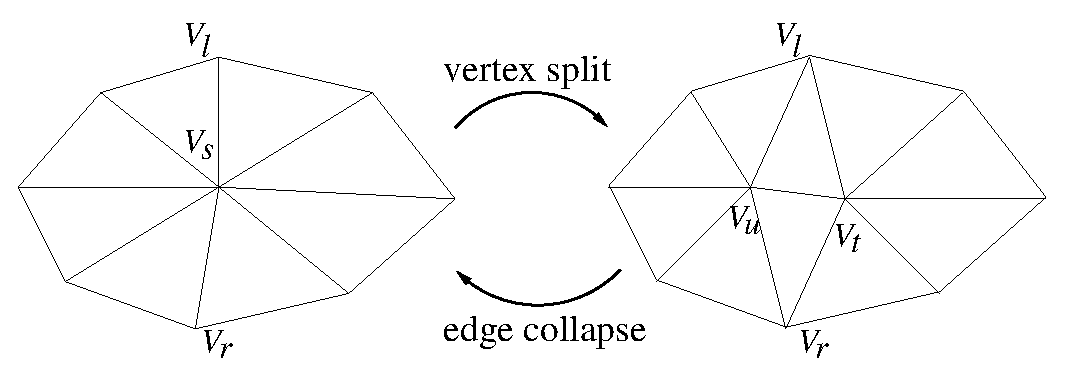
\epsfig{file =split.eps, height = 0.9in}
    \caption{%Screen area of two vertices: v1 and v2.
    Vertex split and edge collapse. 
    \label{split}}
    \end{figure}
    
    In progressive streaming, the quality of the mesh on the receiver
    increases over time, and plotting this quality versus time gives us a \emph{quality curve}. 
    Because vertex splits contribute differently
    to the quality,
    the quality curve depends on the decoding order of the vertex splits,
    which in turn depends on the sending order of the vertex splits.
    Therefore, it is important to choose a sending order so that the 
    quality on the receiver increases as fast as possible.
    This problem is the main objective of our research. 
    %which is the main difference between progressive mesh streaming and
    %video streaming. This difference introduces some new research problems.
    %In my thesis, three of them are considered.
       
    A natural method is to send vertex splits in the descending order of their contribution to the quality of the received mesh. This strategy, however, is not always optimal, 
    because dependency also plays an important role,
    especially when the mesh is transmitted over a lossy network.
    
    The progressive coding of meshes introduces dependencies among 
    the vertex splits, and the descendants cannot be decoded
    before their ancestors are all decoded. Therefore, 
    when a progressive mesh is transmitted over a lossy network,
    a packet loss will disable the decoding of the following
    vertex splits if they depend on this lost packet. 
    These successfully received vertex splits cannot be 
    decoded until the lost packet is successfully retransmitted. 
    %(we assume that once a packet is detected lost, it 
    %will be retransmitted immediately).
    %Therefore, sending vertex splits that are independent with 
    %the lost packet before the retransmission can improve
    %the quality curve. 
    Hence, the effect of dependency needs to
    be considered in choosing the sending order of vertex splits. 
    To find the effect of dependency
    is non-trivial as the packet loss happens randomly.
    In Section \ref{c:model}, we propose
    an analytical model to quantify the effect of dependency on
    the quality curve.
    
    To further improve the quality curve,
    we can consider the view-point of the 
    user in deciding the sending order.
    Usually, users can only see a part of a mesh, so sending non-visible data
    before visible data wastes bandwidth. Moreover, the visual contributions of visible
    vertex splits (how much they can improve the rendered image)
    also depend on the view-point of the user.
    Hence, choosing the sending order according to the viewpoint of the user, so called
    \emph{view-dependent streaming}, is a natural choice.
    
    In existing solutions to view-dependent streaming,  the
    sender decides the sending order. This sender-driven protocol has several
    drawbacks. First, it is not scalable to many receivers as the sender has to
    determine the visibility of vertices and sort the visible vertex splits based on their
    visual contributions for each receiver. 
    Second, the sender needs to maintain
    the rendering state of each receiver to avoid sending duplicate data. 
    Due to the stateful design and high computational requirements,
    the sender-driven approach cannot be easily extended to support 
    many receivers with caching proxy and peer-to-peer system,
    two common solutions to scalability. 
    %It is not realistic to require each cache or peer to provide much CPU time and memory. 
    %Furthermore, a cache or peer might not have the complete mesh.

    In Section \ref{c:view}, we propose a receiver-driven protocol to 
    improve the scalability. In our protocol, the receiver decides the sending order
    and explicitly requests the vertex splits, 
    while the sender simply sends the data requested.
    The sending order is computed at the receiver  by estimating the visibility
    and visual contributions of the refinements, even before receiving them,
    with the help of GPU.

    The receiver-driven protocol significantly reduces the computing cost at the sender,
    but the bandwidth can remain the bottleneck if each receiver receives data
    from the same sender. Peer-to-peer (P2P) technique is a common solution to increase
    the scalability without high cost to increase the number of servers. 
    Applying the P2P technique into progressive mesh streaming system
    is considerably simplified by our receiver-driven protocol since 
    the sender is stateless and free of expensive computations.
    Whereas, the implementation is still challenging because the flexibility
    of choosing the sending order of 
    vertex splits increases the difficulty of sharing data among peers. 
    
    In P2P mesh streaming, users %may be interested in different
    %part of the mesh at different level of details.  Each 
    may choose to look at different facets, or zoom into different level.
    Therefore, each peer may choose a unique sending order of
    vertex splits. As a result, it is difficult for a peer to keep receiving
    needed data from another peer for a long time, and  
    a peer would have to continuously 
    look for peers to retrieve the mesh data from, which may introduce large
    message overhead.
    %, as the peer's
    %viewpoint and level of details change over time.  
    How to reduce the message overhead then becomes
    %the overhead in this process is 
    one of the main challenges for
    P2P mesh streaming. In Section \ref{c:p2p}, we introduce our current study on how to 
    implement a P2P mesh streaming system based on our receiver-driven protocol.
\section{Related Work}
    Since Hoppe proposed progressive mesh in 1996 \cite{237216}, many studies have
    investigated the streaming of progressive meshes, but most of them assume that the mesh
    is sent in a fixed order. Gu and Ooi \cite{Gu:Packetization} first consider choosing 
    a sending order to reduce the dependency so that the quality curve can be 
    improved. In our study \cite{cheng07analytical}, 
    we consider both the dependency and the contributions of the 
    vertex splits and quantitatively show the effect of dependency.
    
    Many studies of view-dependent streaming of progressive mesh exist, but all of
    them let the sender decide the visibility and the sending order. In these papers,
    we learn most from the work of Kim et al. \cite{kim01truly,multiresolution:kim}.
    We adapt their truly selective method into our
    system both to reduce dependency and to enable implicitly embedding the identification number 
    into the vertex splits.  
    
    P2P streaming of 3D scenes is studied by Hu et al. \cite{Hu2008}, 
    but in their system a single object is still sent in a fixed order.
    In this thesis, we focus on how to send each object in a view-dependent order
    based on our receiver-driven protocol.  
    
\section{An Analytical Model of \\Progressive Mesh Streaming}
\label{c:model}
    In streaming of progressive mesh, we want to choose a sending order of 
    vertex splits so that the quality increases as quickly as possible.
    Hence, we 
    evaluate a sending order based on the quality curve it generates.
    Whereas, streaming of progressive mesh over a lossy network generates a
    random quality curve due to the random packet loss, and the uncertainty of 
    the quality curve increases the difficulty to compare different sending orders. 
    %based on the quality curves. 
    Therefore, we propose an analytical model to
    predict the average quality curve, i.e. the expected value
    of quality at every moment. 
     
    The mesh quality is determined by the decoding time of the vertex
    splits and their contributions to the overall mesh quality.    
    The decoding time of a vertex split depends on its receiving time and the 
    receiving time of its all ancestors. The receiving time of a vertex split
    in turn depends on its sending time and how many times it is 
    transmitted. %The computation is non-trivial since 
    %All these variables are random %The %decoding time of a vertex is a random variable 
    %because packet losses happen randomly, so we need to find their expected values.
    %of the decoding time of each vertex split. 
    
    %Based on probability theory, 
    Our model gives an expression for the expected
    decoding time, given the dependencies among the vertex splits and the network
    condition (including loss probability).
    From this expression, we can efficiently know both the expected 
    value and the distribution of the decoding time of each
    vertex split before transmission. Consequently, 
    %To measure the decoded quality at a given time, we propose
    %a metric based on the contribution of decoded vertex splits to the
    %decoded mesh quality.  This decoded mesh quality can be computed 
    %once we know the expected decoding time of a vertex split
    %and its contribution.
    we can analytically 
    evaluate different sending orders 
    %strategies for streaming
    %a progressive mesh 
    efficiently without simulations.   
    Hence, our model can help in developing a sending
    strategy to improve the quality curve 
    during transmission. % to improve the quality.
    Furthermore, we derive closed-form expressions in two extreme cases,
    providing insights to the importance of dependencies on the
    decoded mesh quality. The main insight is that if each lost packet
    is immediately retransmitted upon the packet loss is detected, 
    then the dependencies only matters in the first several round trip times. 
    Therefore, the effect of dependency is only significant in the applications
    requiring high interactivity. The details can be found in our paper
    \cite{cheng07analytical}. 
   
\section{Receiver-Driven Protocol}
\label{c:view}
    %Receiver-driven protocol can help to reduce the resource usage of the server and 
    %stateless design of the server facilitates the application of caching proxy and 
    %peer-to-peer techniques, but
    Another important factor in choosing the sending order is the view-point of the user.
    We can improve the quality quicker by considering users' view-points. 
    All existed systems let the sender decide the sending order for each receiver, but
    this sender-driven approach is not scalable to a large number of clients. 
    To address this problem, we 
    propose a receiver-driven protocol. 
    Implementing the receiver-driven protocol, however, is non-trivial. 
    First, the receiver has to decide the visual contribution
    of a vertex split before receiving it.
    Second, the receiver needs to know the unique ID (identification number)
    of each vertex so that it
    can explicitly request data to split it. 
    Explicitly
    including the IDs in the vertex splits is not appropriate as it will significantly
    increase the data size.
    
    For the first difficulty, we find that
    although it is difficult for the receiver to accurately measure
    the visual importance of a vertex split before receiving it, estimation suffices
    in our scheme. In current implementation, we estimate
    the visual importance of a vertex splits based on
    \begin{figure}
    \centering
    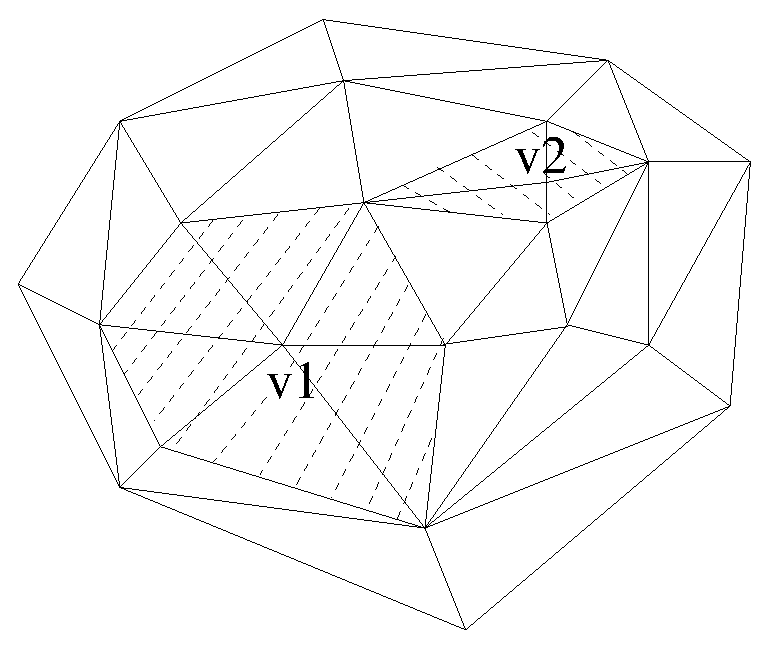
\epsfig{file =screen_area.eps, height = 1.2in}
    \caption{%Screen area of two vertices: v1 and v2.
    Rendered image on the receiver's screen. 
    The shaded are the screen area of vertex $V_1$ and vertex $V_2$.
    \label{screen_area}}
    \end{figure}
     %We use 
    its screen area -- the screen-space area of all the neighbor faces of
    a vertex in the rendered image 
    (see Figure \ref{screen_area}).
    The rationale is that if the screen area of a vertex ($V_1$ in Figure \ref{screen_area}) 
    is larger, it is likely the quality can
    be improved more by splitting this vertex. 
    Moreover, the screen-space area can be efficiently
    computed with the help of the GPU.
    
    To uniquely identify each vertex, we borrow the idea from Kim and Lee \cite{kim01truly}.
    In this system,
    all IDs can be deduced by the receiver without any extra information. The IDs of the vertices
    in the base mesh are their sequence numbers. The IDs of the children can be derived from the
    ID of their parent by appending a digit '0' (left child) or '1' (right child).
    
    Then, based on these two solutions, we propose a receiver-driven protocol in which 
    the receiver initiates the transmission by sending a request. Then the sender sends back
    the whole base mesh. The receiver decides the visibility and requests the vertex splits for 
    the visible vertices in the descending order of the 
    screen-space area. If the view point changes, the visual importance will
    be re-computed and a new list of vertex splits will be requested. More details can be found
    in our paper \cite{Cheng2008}.
    
    Because the visibility determination and state maintenance are all done by the receivers, 
    the sender in our receiver-driven protocol is stateless and free of complex computation
    (the CPU cost is reduced by $24\%$ in our experiment). 
    Further, caching proxy and P2P streaming systems can be applied to improve
    the scalability without adding more servers.  
   
\section{Peer-to-Peer Streaming Progressive Meshes}
\label{c:p2p}
    The receiver-driven protocol introduced in Section \ref{c:view} simplifies the 
    implementation of the P2P view-dependent streaming of progressive meshes.
    Some significant modifications and extensions, however, need to be done to apply the 
    protocol in a P2P mesh streaming system.
    
    %A common question in peer-to-peer systems is that how a peer knows which peer to request for  
    %needed data. 
    The interactive nature of view-dependent streaming of progressive mesh requires
    low latency. Moreover, in a P2P mesh streaming system, because peers 
    need to frequently look for new peers to retrieve data, the searching time
    cannot be amortized. Hence, reducing the searching time is crucial in progressive
    mesh streaming. One common approach to reduce the latency
    is that each peer advertises its contents periodically
    to other peers. Each peer then knows
    who has the chunk it needs and send the corresponding request without inquiring.
    %To achieve this objective, each peer needs to advertise their contents periodically
    %to other peers. 
    But when the number of peers is large,
    the advertisement packets may overwhelm the whole network. 
    A possible solution is to group the receivers having similar interest together and
    confine the advertisement of contents among peers in the same group to reduce the message
    overhead. 
    
    %Furthermore, we need to increase the size of data unit to be request in 
    %a peer-to-peer mesh streaming system. 
    %In our paper \cite{Cheng2008}, the receiver requests for individual vertex splits explicitly.
    %This design is not appropriate in P2P streaming. 
    %First, since a packet can comprise
    %many vertex splits,
    %the requests occupy a large proportion of the up-link bandwidth,
    %which is precious in P2P streaming since the up-link bandwidth
    %should be used for sharing data with other peers. 
    %Second, the data packet needs to be generated dynamically at the
    %sender whenever a request is received, increasing
    %both computation overhead and delay. 
    
    To address the above problems, we proposed a hierarchical grouping system.
    First, we adapt our receiver-driven protocol to the concept of chunk,
    commonly used in P2P systems.
    Our chunk is of much finer granularity, to allow each peer
    the flexibility of retrieving only the visible segments of a mesh.
    Each chunk has the size of one packet in our implementation, consisting of 
    multiple vertex splits, although we can easily generalize it to
    large chunks. A peer sends a chunk ID to request for a set of vertex splits.
    Once a chunk is received, 
    all the vertex splits in this chunk are decoded.
    %We sacrifice some flexibility in choosing vertices,
    %but significantly reduces the up-link bandwidth requirement. 
    %and frees the peers from online generating packets.
    %since
    %now only one chunk ID is needed to request a set of vertices.
    %The cost of searching for peers to retrieve data is also reduced.
    %Furthermore, since grouping vertex splits into chunks can be done in the server
    %offline, no computation cost and delay are needed for peers to
    %do online packetization. 
    
    The question now is that how a peer knows which chunk to request
    and which group to join when it decides to refine a certain segment of a mesh.  
    One naive solution is to store the chunk ID and group ID together with vertices,
    but this method adds additional overhead.
    %(suppose the chunk
    %ID is 2 bytes and in our mesh encoding a vertex split just needs 3-4 bytes, the overhead is
    %more than 50\%).  
    Another method is to organize the mesh into a
    hierarchy of bounding boxes and to generate chunks and groups based on the bounding boxes.
    %The chunk ID can thus be deduced from the vertex coordinates.
    Whereas, since a vertex in a bounding box might have ancestors in other bounding
    boxes, this method increases dependencies among the chunks, which might
    delay the decoding of some received vertices until other chunks have been received.
      
    In our hierarchical grouping system, 
    we define chunks and groups based on vertex dependencies. In brief, 
    a chunk comprises vertices having common ancestor and a group comprises
    chunks having common ancestors.   
    \begin{figure}[t]
    \centering
    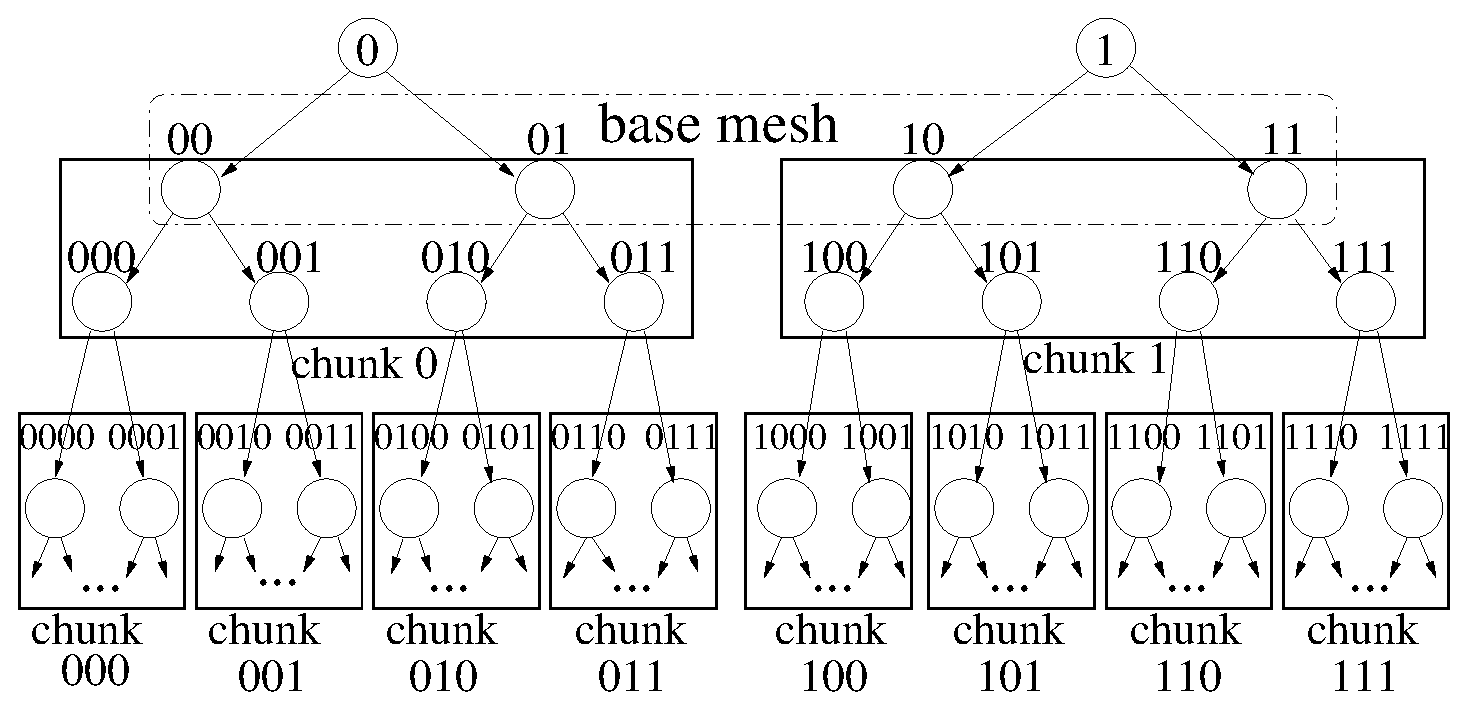
\epsfig{file = packetize.eps, height = 1.5in, width = 3.3in}
    \caption{A simple hierarchical grouping system.
    \label{packetize}}
    \end{figure}
    Figure \ref{packetize} is a simple example and more details are omitted 
    due to the space limit here.    
    
    The main advantages of the hierarchical grouping system are as follows.
    First, it fits the dependency among the vertex splits
    well, so the packetization will not increase the dependency
    among the chunks.
    Second, since all vertices in a chunk have a common ancestor, 
    they are connected and typically close to each other.
    Hence, our hierarchical group
    incorporates spatial locality. 
    Third, the group ID and chunk ID are implicitly
    coded with the vertex ID, so they can be deduced by the receiver without any extra data.

    We are still working on this problem. %This study is still ongoing. 
    %According to current results, the hierarchical 
    %grouping system works well. 
    Our current experimental results show that the hierarchical grouping system works well.
    %With this system, 
    We can reduce the server 
    overhead by about 90\% at the cost of 10\% message overhead. Meanwhile, the latency is
    acceptable. 
    %server overhead with introducing 10\% message overhead.        
\section{Future Plan}
\label{c:conclude}
    We have several plans to improve our current study.
    First, we plan to adapt our analytical model to the real network,
    as currently the analytical
    model is based on simulations. It is challenging since the packet loss in the real
    network is complex. 
    Second, we want to improve our receiver-driven protocol with
    a better method to estimate the visual contributions of vertex splits. A candidate 
    is to consider the complexity of the shape of the neighborhood \cite{estimating:chen}.
    Third, we will continue our research on the P2P mesh streaming system. 
    %The main objective is to 
    %reduce the server overhead as much as possible, but meanwhile the response time and the message
    %overhead should be kept low. 
    Some of the main research problems are:
    %(1) how to help peers find source without high message head;
    (1) how we can reduce the switch delay since switching happens frequently;
    and (2) whether the push-based method can be used in the mesh streaming
    system to reduce the response time.  
\begin{thebibliography}{50}
\vspace*{0.7mm}
\footnotesize
\bibitem{estimating:chen}
Y.~Chen and H.~Sundaram.
\newblock Estimating complexity of 2{D} shapes.
\newblock In {\em Proceeding of IEEE 7th Workshop on Multimedia Signal
  Processing, 2005}, pages 1--4, Shanghai, China, October 2005.

\bibitem{Cheng2008}
W.~Cheng and W.~T. Ooi.
\newblock Receiver-driven view-dependent streaming of progressive mesh.
\newblock In {\em Proceedings of NOSSDAV'08}, Brauschweig, Germany, May 2008.

\bibitem{cheng07analytical}
W.~Cheng, W.~T. Ooi, S.~Mondet, R.~Grigoras, and G.~Morin.
\newblock An analytical model for progressive mesh streaming.
\newblock In {\em Proceedings of MULTIMEDIA '07}, pages 737--746, Augsberg,
  Germany, September 2007.

\bibitem{Gu:Packetization}
Y.~Gu and W.~T. Ooi.
\newblock Packetization of 3{D} progressive meshes for streaming over lossy
  networks.
\newblock In {\em Proceedings of ICCCN'05}, San Diego, CA, October 2005.

\bibitem{237216}
H.~Hoppe.
\newblock Progressive meshes.
\newblock In {\em Proceeding of SIGGRAPH '96}, pages 99--108, New Orleans, USA,
  August 1996.

\bibitem{Hu2008}
S.-Y. Hu, T.-H. Huang, S.-C. Chang, W.-L. Sung, J.-R. Jiang, and B.-Y. Chen.
\newblock {FLoD}: A framework for peer-to-peer {3D} streaming.
\newblock In {\em Proceedings of IEEE INFOCOM}, April 2008.

\bibitem{multiresolution:kim}
J.~Kim, S.~Choe, and S.~Lee.
\newblock Multiresolution random accessible mesh compression.
\newblock {\em Computer Graphics Forum}, 25(3):323--331, September 2006.

\bibitem{kim01truly}
J.~Kim and S.~Lee.
\newblock Truly selective refinement of progressive meshes.
\newblock In {\em Proceedings of Graphics Interface 2001}, pages 101--110, June
  2001.

\end{thebibliography}
%\bibliographystyle{abbrv}
%\bibliography{symposium}
\end{document}
